\chapter{The full pipeline}
\label{chap:pipeline}

\section{Pipeline order}

As described in chatper~\ref{chap:basicpipeline} and in figure~\ref{fig:pipeline:order} (reported here as figure~\ref{fig:pipeline:order-again} for convenience), the pipeline can be implemented either in the blue or in the orange order.

From the results of chatper~\ref{chap:3dlink}, the \linkDDD* (in the orange order) was quite faster than the \linkDD*: a faster step implies less computation resources used, which leaves more available for the most intensive tasks.
The other benefit of the orange pipeline is that the linking is performed in 3D, where more information are available.
In particular, it was noticed relatively often that the \match* step would reconstruct bubbles belonging to the same 2D tracklet at different depths, creating a sudden jump in the 3D trajectory, indicating an error.
Instead, when the \linkDDD* was used, the results were more coherent.
As such, the orange order was chosen for the pipeline.

\begin{figure}
	\centerline{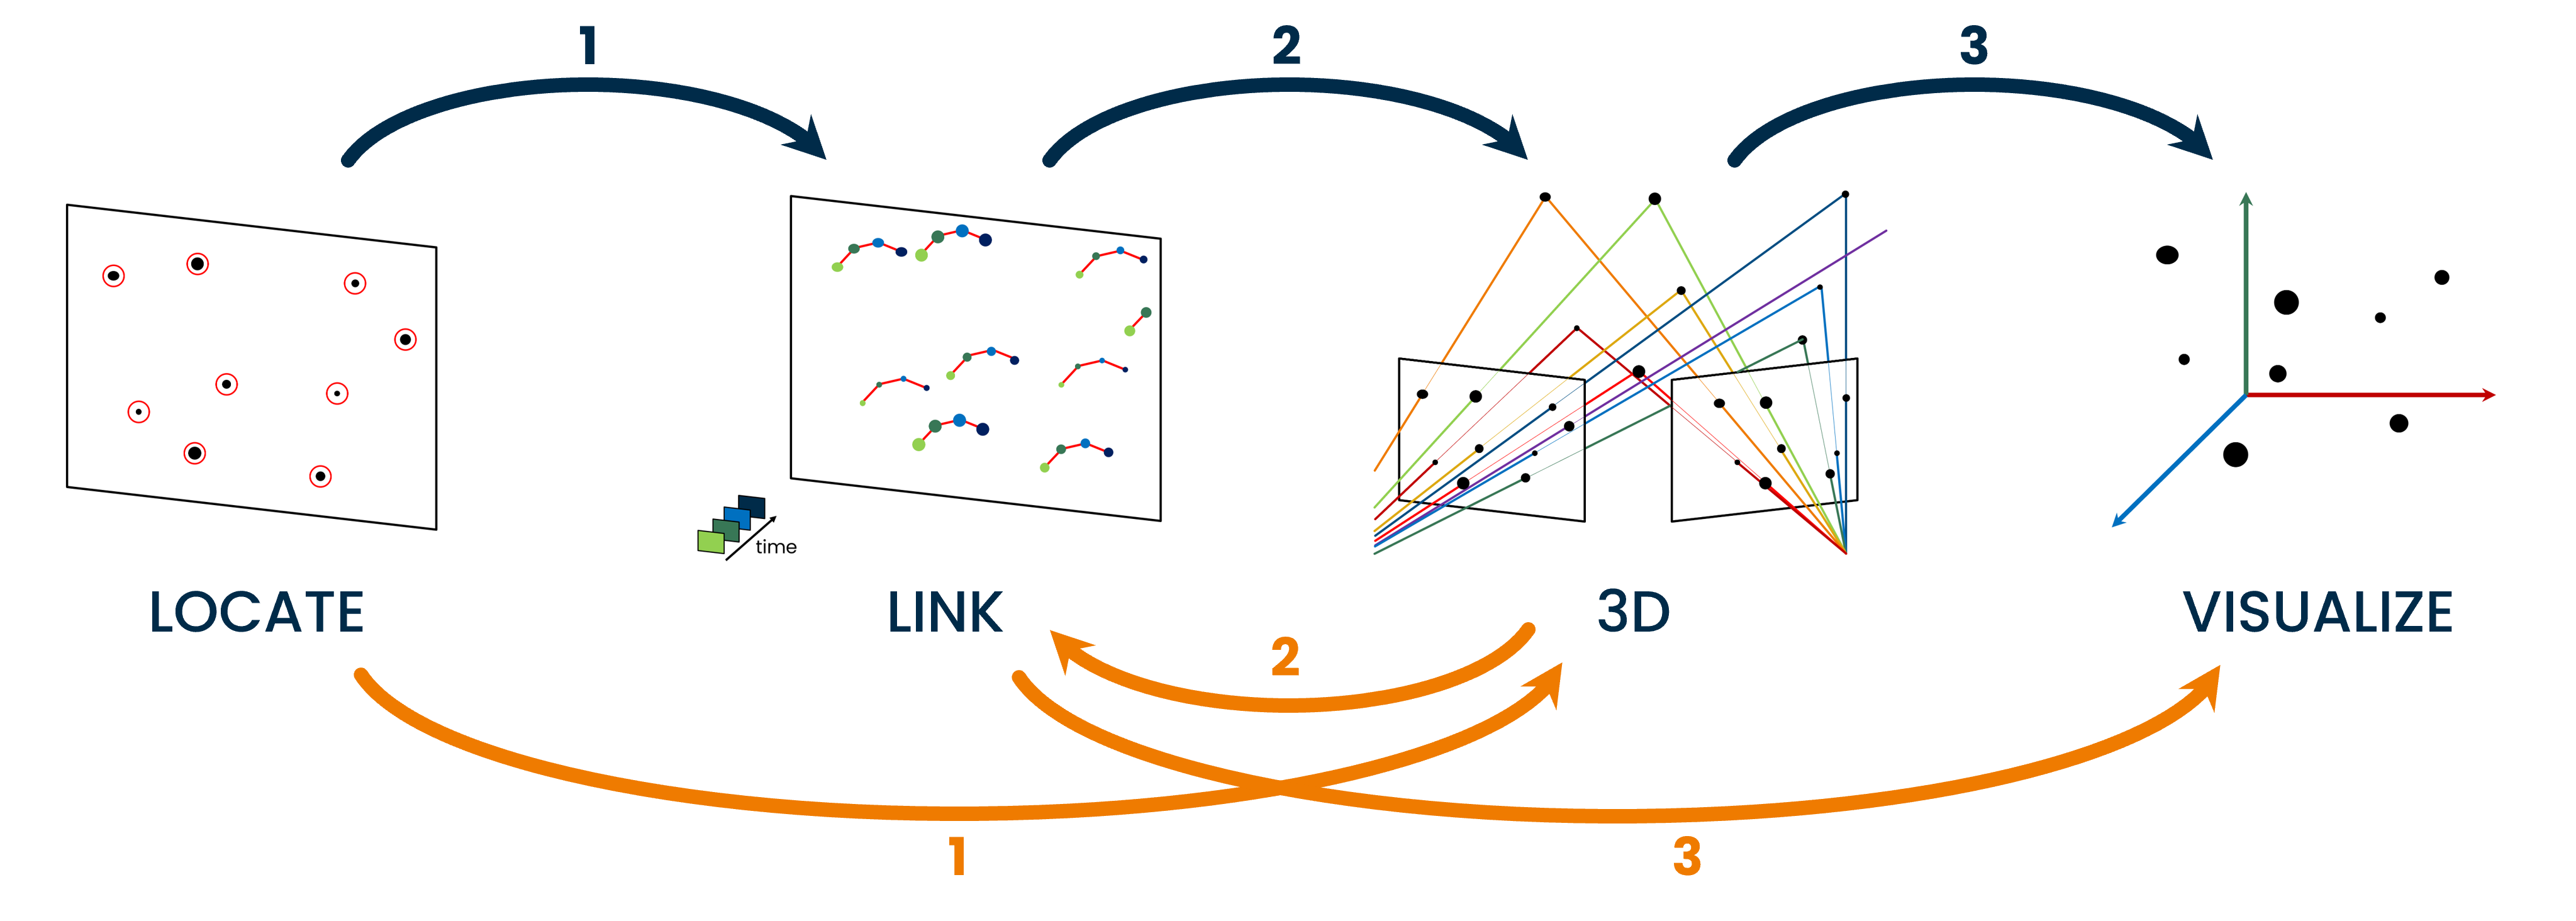
\includegraphics[width=\textwidth]{images/pipeline-orders.png}}
	\caption{\centering The two different orders in which the pipeline can be executed}
	\label{fig:pipeline:order-again}
\end{figure}

\section{Implementation}

The pipeline is implemented on the operating system as a set of processes, to fully use all the cores of the CPU.
Simpler threads would not be equivalent, since all Python threads are executed on the same CPU core.
The communication among the processes is realized by means of shared memory locations, where the input/output arrays are stored in a shared way.

The different processes are organized as follows:
\begin{itemize}
	\item the \locate* step is performed by its own process, that:
	      \begin{itemize}[topsep=0pt]
		      \itemsep 0em
		      \item loads the images either from the cameras or from file;
		      \item finds the bubbles using the \texttt{findContours} function;
		      \item launches and waits for the GPU computation of the moments.
	      \end{itemize}
	\item a process runs the \match* step, that:
	      \begin{itemize}[topsep=0pt]
		      \itemsep 0em
		      \item waits until new data is available from the \locate* step;
		      \item computes the first guess of matching;
		      \item computes the median displacement;
		      \item refines the first guess with the computed medians;
		      \item uses the matches to reconstruct 3D coordinates;
	      \end{itemize}
	\item the \link* (\linkDDD*) step is executed in another process, that:
	      \begin{itemize}[topsep=0pt]
		      \itemsep 0em
		      \item waits until new data is available from the \match* step;
		      \item performs the linking;
	      \end{itemize}
	\item if enabled, the \visual* step is run by a separate process, that:
	      \begin{itemize}[topsep=0pt]
		      \itemsep 0em
		      \item activates a new virtual environment, since \texttt{Open3D} requires a \texttt{NumPy} version not compatible with the rest;
		      \item runs the visualization script, that constantly checks for new values, displays them and responds to the user input.
	      \end{itemize}
	\item if enabled, a final debug process constantly updates the output in the terminal, writing the total number of frames processed by each step.
\end{itemize}
The different waits are realized as a loop that performs a 0.5s sleep until more data is available.
